\documentclass[10pt]{beamer}\usepackage[]{graphicx}\usepackage[]{color}
%% maxwidth is the original width if it is less than linewidth
%% otherwise use linewidth (to make sure the graphics do not exceed the margin)
\makeatletter
\def\maxwidth{ %
  \ifdim\Gin@nat@width>\linewidth
    \linewidth
  \else
    \Gin@nat@width
  \fi
}
\makeatother

\definecolor{fgcolor}{rgb}{0.345, 0.345, 0.345}
\newcommand{\hlnum}[1]{\textcolor[rgb]{0.686,0.059,0.569}{#1}}%
\newcommand{\hlstr}[1]{\textcolor[rgb]{0.192,0.494,0.8}{#1}}%
\newcommand{\hlcom}[1]{\textcolor[rgb]{0.678,0.584,0.686}{\textit{#1}}}%
\newcommand{\hlopt}[1]{\textcolor[rgb]{0,0,0}{#1}}%
\newcommand{\hlstd}[1]{\textcolor[rgb]{0.345,0.345,0.345}{#1}}%
\newcommand{\hlkwa}[1]{\textcolor[rgb]{0.161,0.373,0.58}{\textbf{#1}}}%
\newcommand{\hlkwb}[1]{\textcolor[rgb]{0.69,0.353,0.396}{#1}}%
\newcommand{\hlkwc}[1]{\textcolor[rgb]{0.333,0.667,0.333}{#1}}%
\newcommand{\hlkwd}[1]{\textcolor[rgb]{0.737,0.353,0.396}{\textbf{#1}}}%
\let\hlipl\hlkwb

\usepackage{framed}
\makeatletter
\newenvironment{kframe}{%
 \def\at@end@of@kframe{}%
 \ifinner\ifhmode%
  \def\at@end@of@kframe{\end{minipage}}%
  \begin{minipage}{\columnwidth}%
 \fi\fi%
 \def\FrameCommand##1{\hskip\@totalleftmargin \hskip-\fboxsep
 \colorbox{shadecolor}{##1}\hskip-\fboxsep
     % There is no \\@totalrightmargin, so:
     \hskip-\linewidth \hskip-\@totalleftmargin \hskip\columnwidth}%
 \MakeFramed {\advance\hsize-\width
   \@totalleftmargin\z@ \linewidth\hsize
   \@setminipage}}%
 {\par\unskip\endMakeFramed%
 \at@end@of@kframe}
\makeatother

\definecolor{shadecolor}{rgb}{.97, .97, .97}
\definecolor{messagecolor}{rgb}{0, 0, 0}
\definecolor{warningcolor}{rgb}{1, 0, 1}
\definecolor{errorcolor}{rgb}{1, 0, 0}
\newenvironment{knitrout}{}{} % an empty environment to be redefined in TeX

\usepackage{alltt}%
\usetheme{Boadilla}
\usecolortheme{seahorse}

\usepackage[utf8]{inputenc}%


\usepackage[normalem]{ulem}%strikeout
 

% graphics
%% Figures %%%%%%%%%%%%%%%%%%%%%%%%%%%%%%%%%%%%%%%%%%%%%%%%%%
\usepackage{graphicx}
\usepackage{xcolor}%for color mixing

\usepackage{amsmath}%
\usepackage{amsfonts}%
\usepackage{amssymb}%
\usepackage{graphicx}

\usepackage{tikz}
\usetikzlibrary{calc}

%%%%%%%%%%%%%%%%%%%%%%%%%%%%%%%%%%%%%%%%%%%%%%
%%%%%%%%%%%%%%%%% Doc info %%%%%%%%%%%%%%%%%%%
\title[\textbf{Generalized linear models:}]{Generalized Linear Models (GLMs)}
\date{\today}

%%%%%%%%%%%%%%%%%%%%%%%%%%%%%%%%%%%%
\IfFileExists{upquote.sty}{\usepackage{upquote}}{}
\begin{document}




\begin{frame}
\maketitle
\end{frame}
%%%%%%%%%%%

\AtBeginSection[]
{
  \begin{frame}<beamer>
    \frametitle{}
    \tableofcontents[currentsection,hideothersubsections,subsectionstyle=hide]% down vote\tableofcontents[currentsection,currentsubsection,hideothersubsections,sectionstyle=show/hide,subsectionstyle=show/shaded/hide]
  \end{frame}
}



%%%%%%%%%%%%%%%%%%%%%%%%%%%%%%%%%%%%%%%%%%%%%%%%%%%%%%%%%%%%%%%%%%%
%%%%%%%%%%%%%%%%%%%%%%%%%%%%%%%%%%%%%%%%%%%%%%%%%%%%%%%%%%%%%%%%%%%
\section{Linear model, reminder}

\begin{frame}[fragile]{A simple linear model}
  \textbf{{\color{purple}{Response}} = {\color{blue}{Intercept}} + {\color{red}{Slope}} $\times$ {\color{orange}{Predictor}} + {\color{gray}{Error}}} \\

\begin{knitrout}\small
\definecolor{shadecolor}{rgb}{0.843, 0.867, 0.922}\color{fgcolor}
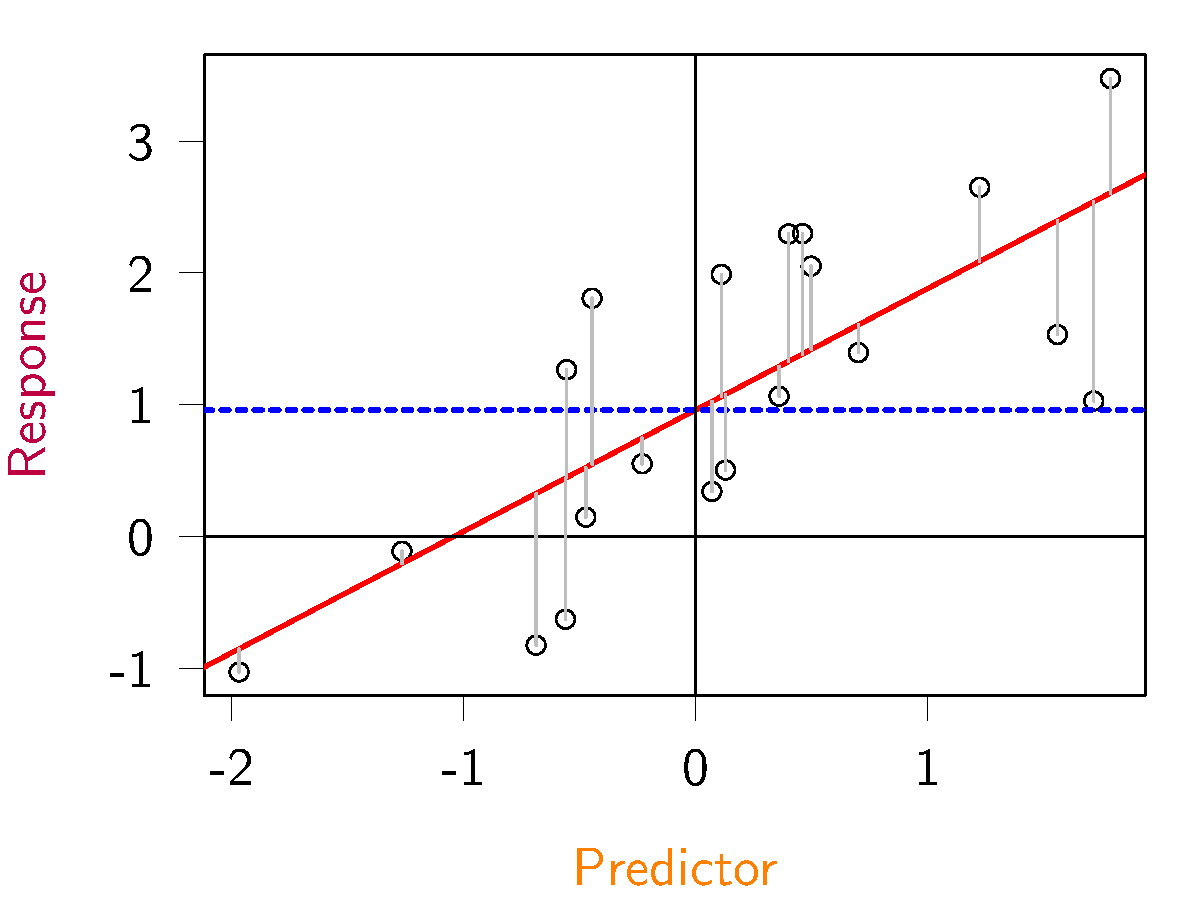
\includegraphics[width=0.8\textwidth,height=0.6\textwidth]{figure/lmprinc-1} 

\end{knitrout}
\end{frame}
%%%%%%%%%%%

\begin{frame}[fragile]{A simple linear model failure: binary data}

\begin{knitrout}\small
\definecolor{shadecolor}{rgb}{0.843, 0.867, 0.922}\color{fgcolor}
\includegraphics[width=0.8\textwidth,height=0.6\textwidth]{figure/binlmprinc-1} 

\end{knitrout}
  
\end{frame}
%%%%%%%%%%%

\begin{frame}{Linear model basic assumptions}
 \begin{block}{}
     \begin{itemize}
      \item Linear combination of parameters (including transformation, polynoms, interactions\dots)\\ \textit{Risk: biologically meaningless}
      \item Predictor not perfectly correlated \\ \textit{Risk: Model won't run, unstable convergence, or huge SE}
       \item {\color{red!20!black}{Little error in predictors}}\\ \textit{Risk: bias estimates (underestimate with Gaussian error)}
       \item {\color{red!50!black}{Gaussian error distribution}}\\ \textit{Risk: Poor predictions}
       \item {\color{red!70!black}{Homoscedasticity (constant error variance)}}\\ \textit{Risk: Over-optimistic uncertainty, unreliable predictions}
       \item {\color{red!99!black}{Independence of error}}\\ \textit{Risk: Bias and over-optimistic uncertainty}
     \end{itemize}
 \end{block}
\end{frame}
%%%%%%%%%%%

\begin{frame}[fragile]{A simple linear model failure: binary data}

\begin{knitrout}\small
\definecolor{shadecolor}{rgb}{0.843, 0.867, 0.922}\color{fgcolor}
\includegraphics[width=0.7\textwidth,height=0.53\textwidth]{figure/binlmprinc2-1} 

\end{knitrout}
  
  \begin{alertblock}{Assumptions violated:}
    Non-Gaussian errors, non-constant error variance, correlated errors
  \end{alertblock}
\end{frame}
%%%%%%%%%%%

\begin{frame}[fragile]{A simple linear model failure: binary data}

\begin{knitrout}\small
\definecolor{shadecolor}{rgb}{0.843, 0.867, 0.922}\color{fgcolor}
\includegraphics[width=0.7\textwidth,height=0.53\textwidth]{figure/binlmprinc3-1} 

\end{knitrout}
  \begin{alertblock}{Practical consequences:}
    Non-sensical predictions, wrong confidence-interval and p-value, extrapolation ALWAYS fails
  \end{alertblock}
\end{frame}
%%%%%%%%%%%

\begin{frame}[fragile]{What we want our model to do}
\begin{knitrout}\small
\definecolor{shadecolor}{rgb}{0.843, 0.867, 0.922}\color{fgcolor}
\includegraphics[width=0.7\textwidth,height=0.53\textwidth]{figure/binglmprinc-1} 

\end{knitrout}
    \begin{alertblock}{Good features:}
    Never out of [0,1], variable uncertainty, non-linear trend, close fit
  \end{alertblock}
\end{frame}
%%%%%%%%%%%

\begin{frame}{That is what a Generalized Linear Model does}

\begin{block}{Vocabulary warning}
  \begin{itemize}
    \item General Linear Model (=linear model with several responses, multivariate)
    \item \textbf{Generalized Linear Model (=non-normal errors, and uncertainty dependent on the mean)} 
  \end{itemize}
\end{block}

\pause

\begin{block}{What a GLM is:}
  \begin{enumerate}
    \item A linear function ($y = \mu + \beta x$ \dots)
    \item A probability distribution (Bernouilli, Binomial, Poisson\dots)
    \item A "link function" to convert between the scale of the linear function ($-\infty$ to $+\infty$) and the scale of the data and the probability distribution (often positive integer: 0, 1, 2, 3\dots)
  \end{enumerate}
  A GLM fits a continuous expected response; we observe discrete realizations
\end{block}

\end{frame}
%%%%%%%%%%%

\begin{frame}[fragile]{Logistic regression}
  \begin{itemize}
    \item Binary or proportion data (survival, presence/absence\dots)
    \item Binomial probability distribution ( = Bernouilly if binary data)
    \item Link function often logit: $y=\log(\frac{probability}{1-probability})$
    \item Back-transformation inverse-logit: $probability = \frac{1}{1 + exp(-y)}$
    \item Linear function $y = intercept + slope_1 predictor_1 + slope_2 predictor_2 +$ \dots
  \end{itemize}

\pause
  Binomial (and Bernouilli distribution in R):
\begin{knitrout}\small
\definecolor{shadecolor}{rgb}{0.843, 0.867, 0.922}\color{fgcolor}\begin{kframe}
\begin{alltt}
  \hlstd{bernouilli_random_sample} \hlkwb{<-} \hlkwd{rbinom}\hlstd{(}\hlkwc{n} \hlstd{=} \hlnum{10000}\hlstd{,} \hlkwc{size} \hlstd{=} \hlnum{1}\hlstd{,} \hlkwc{prob} \hlstd{=} \hlnum{0.3}\hlstd{)}
  \hlkwd{hist}\hlstd{(bernouilli_random_sample)}
  \hlkwd{mean}\hlstd{(bernouilli_random_sample);} \hlnum{0.3}
  \hlkwd{var}\hlstd{(bernouilli_random_sample);} \hlnum{0.3}\hlopt{*}\hlstd{(}\hlnum{1}\hlopt{-}\hlnum{0.3}\hlstd{)}
\end{alltt}
\end{kframe}
\end{knitrout}
  \pause
  Logistic regression in R:
\begin{knitrout}\small
\definecolor{shadecolor}{rgb}{0.843, 0.867, 0.922}\color{fgcolor}\begin{kframe}
\begin{alltt}
  \hlkwd{glm}\hlstd{(}\hlkwc{formula} \hlstd{= obs} \hlopt{~} \hlnum{1} \hlopt{+} \hlstd{x,} \hlkwc{family} \hlstd{=} \hlstr{"binomial"}\hlstd{,} \hlkwc{data}\hlstd{=data)}
\end{alltt}
\end{kframe}
\end{knitrout}
  
\end{frame}
%%%%%%%%%%%

\begin{frame}[fragile]{Logistic regression}
  
  %data prep




  \begin{exampleblock}{Exercise}
    \begin{enumerate}
      \item Load \texttt{survivalsize.csv}
      \item Plot survival data. What kind of distribution is it?
      \item Fit a linear model and a logistic model with intercept only. How to interpret the estimate?
      \item Fit a linear regression and a logistic regression of survival on relative size, compare the output
      \item Check the diagnostic plots for both models. Should you be worried?
      \item Extract and visualize a model prediction from both models (use the function predict, and/or do it by hand to practice link-function back-transformation)
    \end{enumerate}
  \end{exampleblock}


\end{frame}
%%%%%%%%%%%

\begin{frame}{Logistic regression: trivia}

  \begin{itemize}[<+->]
    \item Many other link-functions, e.g. probit has nice properties to measure selection
    \item logit and inverse-logit functions in boot and mixtools packages
    \item exp(slope) is an odd-ratio 
    \item GLMs on binary data are more (or equally) powerful than proportion data
  \end{itemize}
\end{frame}
%%%%%%%%%%%%%%%%%%%%%%%%%%%%%%%%%%%%%%%%%%%%%%%%%%%%%%%%%%%%%%%%
%%%%%%%%%%%%%%%%%%%%%%%%%%%%%%%%%%%%%%%%%%%%%%%%%%%%%%%%%%%%%%%%

\begin{frame}[fragile]{Poisson regression}
  \begin{itemize}
    \item Count data
    \item Poisson distribution
    \item Link function: logarithm
    \item Inverse link function: exponential
    \item Linear function $y = intercept + slope_1 predictor_1 + slope_2 predictor_2 +$ \dots
  \end{itemize}
  
  \pause
  Poisson distribution in R:
\begin{knitrout}\small
\definecolor{shadecolor}{rgb}{0.843, 0.867, 0.922}\color{fgcolor}\begin{kframe}
\begin{alltt}
  \hlstd{poisson_random_sample} \hlkwb{<-} \hlkwd{rpois}\hlstd{(}\hlkwc{n} \hlstd{=} \hlnum{10000}\hlstd{,} \hlkwc{lambda} \hlstd{=} \hlnum{4}\hlstd{)}
  \hlkwd{hist}\hlstd{(poisson_random_sample)}
  \hlkwd{mean}\hlstd{(poisson_random_sample)}
  \hlkwd{var}\hlstd{(poisson_random_sample)}
\end{alltt}
\end{kframe}
\end{knitrout}
  \pause
  Poisson regression in R:
\begin{knitrout}\small
\definecolor{shadecolor}{rgb}{0.843, 0.867, 0.922}\color{fgcolor}\begin{kframe}
\begin{alltt}
  \hlkwd{glm}\hlstd{(}\hlkwc{formula} \hlstd{= obs} \hlopt{~} \hlnum{1} \hlopt{+} \hlstd{x,} \hlkwc{family} \hlstd{=} \hlstr{"poisson"}\hlstd{,} \hlkwc{data} \hlstd{= data)}
\end{alltt}
\end{kframe}
\end{knitrout}
\end{frame}
%%%%%%%%%%%

\begin{frame}[fragile]{Poisson regression}


  
  
  \begin{exampleblock}{Exercise}
    \begin{enumerate}
      \item Load the data reproduction.csv
      \item Plot reproduction data, calculate the mean and variance. 
      \item Overlay a Gaussian distribution of same mean and variance, does it fit?
      \item Fit an compare a lm and a Poisson glm of reproduction on size 
      \item Check the diagnostic plots for both models. Should you be worried?
      \item Extract and visualize a model prediction from both models (use the function predict, and/or do it by hand to practice link-function back-transformation)
      \item Before GLMs, researchers used to log-transform the data and fit linear models. What are the problems with this approach?
    \end{enumerate}
  \end{exampleblock}
  


\end{frame}
%%%%%%%%%%%

\begin{frame}[fragile]{Poisson regression: over-dispersion}
  \begin{alertblock}{Sadly, simple Poisson models are almost always wrong in natura}
    \begin{itemize}[<+->]
      \item Poisson assumes: expected value = values variance
      \item True if all the sources of variation are in the model (almost impossible)
      \item Main risk:
        \begin{itemize}
          \item underestimate uncertainty 
          \item anti-conservative p-values
          \item find effects that are not real
        \end{itemize}
      \item Opposite risk rare but possible (e.g., bird clutch size)
      \item Solutions: relax mean/variance relationship
        \begin{itemize}
          \item Negative-binomial distribution 
          \item Quasi-Poisson (multiplicative over-dispersion)
          \item Observation-level random effect (additive over-dispersion)
        \end{itemize}
      \item \textbf{You should NEVER use glm(family $=$ poisson) again!}
    \end{itemize}
  \end{alertblock}
  
\end{frame}
%%%%%%%%%%%

 \begin{frame}[fragile]{Poisson regression: over-dispersion demonstrated}

\begin{knitrout}\small
\definecolor{shadecolor}{rgb}{0.843, 0.867, 0.922}\color{fgcolor}\begin{kframe}
\begin{alltt}
   \hlkwd{set.seed}\hlstd{(}\hlnum{123}\hlstd{)} \hlcom{# random seed}
   \hlstd{x} \hlkwb{<-} \hlkwd{rnorm}\hlstd{(}\hlnum{100}\hlstd{)} \hlcom{# predictor with no effect}
   \hlstd{y} \hlkwb{<-} \hlkwd{exp}\hlstd{(}\hlopt{-}\hlnum{1} \hlopt{+} \hlkwd{rnorm}\hlstd{(}\hlnum{100}\hlstd{,} \hlnum{0}\hlstd{,} \hlnum{2}\hlstd{))} \hlcom{# variation of unknown origin}
   \hlstd{obs} \hlkwb{<-} \hlkwd{sapply}\hlstd{(y,} \hlkwc{FUN} \hlstd{=} \hlkwa{function}\hlstd{(}\hlkwc{y}\hlstd{)\{}
     \hlkwd{rpois}\hlstd{(}\hlkwc{n} \hlstd{=} \hlnum{1}\hlstd{,} \hlkwc{lambda} \hlstd{= y)\})} \hlcom{# generate Poisson data}

   \hlcom{#plot(x, obs) # visualize data}
   \hlstd{glm2} \hlkwb{<-} \hlkwd{glm}\hlstd{(obs} \hlopt{~} \hlstd{x,} \hlkwc{family} \hlstd{=} \hlstr{"poisson"}\hlstd{)} \hlcom{#fit Poisson regression}
   \hlstd{sglm2} \hlkwb{<-} \hlkwd{summary}\hlstd{(glm2)} \hlcom{#look at the summary}
   \hlstd{sglm2}\hlopt{$}\hlstd{coefficients[}\hlnum{2}\hlstd{,}\hlnum{4}\hlstd{]} \hlcom{# the p-value }
\end{alltt}
\begin{verbatim}
[1] 1.25526e-49
\end{verbatim}
\begin{alltt}
   \hlstd{glm2q} \hlkwb{<-} \hlkwd{glm}\hlstd{(obs} \hlopt{~} \hlstd{x,} \hlkwc{family} \hlstd{=} \hlstr{"quasipoisson"}\hlstd{)} \hlcom{#quasiPoisson regression}
   \hlstd{sglm2q} \hlkwb{<-} \hlkwd{summary}\hlstd{(glm2q)} \hlcom{#summary}
   \hlstd{sglm2q}\hlopt{$}\hlstd{coefficients[}\hlnum{2}\hlstd{,}\hlnum{4}\hlstd{]} \hlcom{# p-value}
\end{alltt}
\begin{verbatim}
[1] 0.09476039
\end{verbatim}
\end{kframe}
\end{knitrout}
 
\end{frame}
%%%%%%%%%%%

\begin{frame}[fragile]{Poisson regression: over-dispersion demonstrated}


 Maybe just bad luck?
\begin{exampleblock}{Exercise}
  Write a for loop to look at the distribution of p-values
\end{exampleblock}

\begin{knitrout}\small
\definecolor{shadecolor}{rgb}{0.843, 0.867, 0.922}\color{fgcolor}\begin{kframe}
\begin{alltt}
    \hlkwd{set.seed}( )
    poisson_pvalues <- \hlkwd{vector}(length = 1000)
    quasipoisson_pvalues <-
    \hlkwd{for}(i in  )
    \{
      simulation + poisson and quasipoisson GLMs
    \}
    \hlkwd{hist}( )
    \hlkwd{mean}( <0.05)
\end{alltt}
\end{kframe}
\end{knitrout}

% 
%     <<echo=FALSE, eval=FALSE>>=
%     set.seed(123)
%     pvvector <- vector(length = 1000)
%     pvvectorq <- vector(length = 1000)
%     for (i in 1:1000)
%     {
%     x <- rnorm(100)
%     y <- exp(-1 + rnorm(100, 0, 2))
%     obs <- sapply(y, FUN = function(x){rpois(n = 1, lambda = x)})
%     glm2 <- glm(obs ~ x, family = "poisson")
%     sglm2 <- summary(glm2)
%     pvvector[i] <- sglm2$coefficients[2,4]
% 
%     glm2q <- glm(obs ~ x, family = "quasipoisson")
%     sglm2q <- summary(glm2q)
%     pvvectorq[i] <- sglm2q$coefficients[2,4]
%     }
%     hist(pvvector); mean(pvvector<0.05)
%     hist(pvvectorq) ; mean(pvvectorq<0.05)
%   @
% 

\end{frame}
%%%%%%%%%%%

\begin{frame}{Extras}
  If time allows:
  \begin{itemize}
    \item Jensen inequality
    \item Poisson model in MCMCglmm
  \end{itemize}
\end{frame}
%%%%%%%%%%%
\end{document}
